\chapter{Proof of Concept}
\label{sec:proof_of_concept}

% -------------------------------------------------------------------------------

% parameers: xlabel, center
\newcommand{\fuzzyTreeNode}[2]{
    \begin{tikzpicture}
        \begin{axis}%
            [
                title = {Fuzzy Split: $#1 \leq #2$},
                width=4.5cm,
                height=3cm,
                axis lines=center,
                xlabel={#1},
                x label style={at={(axis description cs:0.9,-0.1)},anchor=north},
                ylabel=$\mu$,
                y label style={at={(axis description cs:0.5,1)},anchor=south},
                xmin=-5,
                xmax=5,
                xtick={},
                xticklabels= {},
                ytick={},
                yticklabels={},
                extra x ticks={0},
                extra x tick labels={#2},
                ymax=1,
                samples=50,
                extra y ticks={1},
                every axis plot/.append style={thick}
            ]
            \addplot[red]  {sigmoid(x,0,-1)};
            \addplot[blue] {sigmoid(x,0,1)};
            \node[anchor=center, red] at (axis cs:-2.9,0.6) {$\mu_{\text{#1smaller#2}}$};
            \node[anchor=center, blue] at (axis cs:3.1,0.6) {$\mu_{\text{#1greater#2}}$};
        \end{axis}

    \end{tikzpicture}
}

\newcommand{\fuzzyTreeLeaf}[1]{
    \begin{tikzpicture}
        \begin{axis}%
            [
                title = {Class: #1},
                width=3.25cm,
                height=2.25cm,
                axis lines=center,
                xlabel={$\text{class}$},
                x label style={at={(axis description cs:0.6,-0.3)},anchor=west},
                ylabel=$\mu$,
                y label style={at={(axis description cs:0.5,1)},anchor=south},
                xmin=-5,
                xmax=5,
                xtick={},
                xticklabels= {},
                ytick={},
                yticklabels={},
                extra x ticks={0},
                extra x tick labels={#1},
                ymax=1,
                samples=10,
                extra y ticks={1},
                every axis plot/.append style={thick}
            ]
            \addplot[black]  {gaussian(x,0,1)};
        \end{axis}

    \end{tikzpicture}
}

% parameers: xlabel, center
\newcommand{\crispTreeNode}[2]{
    \begin{tikzpicture}
        \begin{axis}%
            [
                title = {Crisp Split: $#1 \leq #2$},
                width=4.5cm,
                height=3cm,
                axis lines=center,
                xlabel={#1},
                x label style={at={(axis description cs:0.9,-0.1)},anchor=north},
                ylabel=$\mu$,
                y label style={at={(axis description cs:0.5,1)},anchor=south},
                xmin=-5,
                xmax=5,
                xtick={},
                xticklabels= {},
                ytick={},
                yticklabels={},
                extra x ticks={0},
                extra x tick labels={#2},
                ymin=-0.1,
                ymax=1.1,
                samples=50,
                extra y ticks={1},
                every axis plot/.append style={thick}
            ]
            \addplot[red,domain=-5:-0.6] {step(x,0,-1)};
            \addplot[blue,domain=0.6:5] {step(x,0,1)};
            \addplot[red,domain=0.6:5] {step(x,0,-1)};
            \addplot[blue,domain=-5:-0.6] {step(x,0,1)};

            \node[draw,draw=black,circle,inner sep=1pt,minimum width=3pt,thick] at (axis cs:0,1) {};
            \node[draw,draw=black,circle,inner sep=1pt,minimum width=3pt,thick] at (axis cs:0,0) {};

            \node[anchor=center, red] at (axis cs:-2.9,0.6) {$#1 \leq #2$};
            \node[anchor=center, blue] at (axis cs:3.1,0.6) {$#1 > #2$};
        \end{axis}

    \end{tikzpicture}
}


% -------------------------------------------------------------------------------

This chapter presents a proof of concept for the fuzzy tuning technique. We will develop two different knowledge bases to predict the optimal configurations for \texttt{\gls{mdflexible}} simulations.

As for all fuzzy systems, creating the knowledge base is one of the most complex parts of developing a fuzzy system, as it typically requires a profound understanding of the system to create meaningful rules. Luckily, methods such as data-driven approaches exist to semi-automate this process. This is extremely useful as those methods do not require prior expert knowledge about the system. For a problem as complex as tuning molecular dynamics simulations, it would be extremely hard to create a meaningful knowledge base from scratch. Such data-driven methods provide a good initial set of rules that experts can manually evaluate and adjust if desired. In this work, we will use a decision tree approach proposed by Crockett et al.~\cite{CROCKETT20062809}. This proposed method uses machine learning to first train decision trees on the dataset to create an initial crisp rule base. In the second step, the decision trees are converted into so-called fuzzy decision trees, which can then be used to extract the linguistic variables and fuzzy rules.


\subsection{Decision Trees}

Decision trees are prevalent machine learning algorithms used for classification and regression tasks. They work by recursively partitioning the input using axis-parallel splits so that the resulting subsets are as pure as possible. Concretely, they try to minimize a given impurity metric, such as the Gini impurity $I_G = \sum_{i=1}^{n} p_i(1-p_i)$ or the entropy $H = -\sum_{i=1}^{n} p_i \log_2(p_i)$ of the subsets~\cite{10.5555/2380985}. The probability $p_i$ is the fraction of samples in the subset that belong to class $i$, and $n$ is the total number of classes.

Since decision trees directly partition the input space into regions with different classes, they can also be depicted using their decision surface if the dimensionality allows it. The decision surface of a decision tree is a piecewise constant function that assigns the predicted class label to each point in the input space of the decision tree. An example decision tree and its decision surface are shown in \autoref{fig:decisionTreeExample} and \autoref{fig:decisionBoundaryExample}.

% Image of a decision tree
\begin{multicols}{2}
    \begin{figure}[H] % [H] for HERE
        \centering
        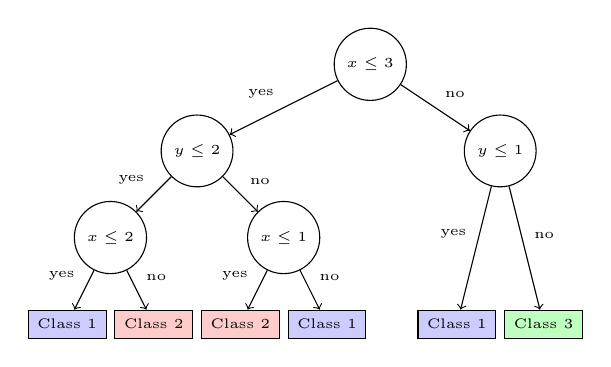
\begin{tikzpicture}[scale=1.1,font=\tiny]
            \node [circle, draw] (A) at (0,0) {$x \leq 3$};
            \node [circle, draw] (B) at (-2,-1) {$y \leq 2$};
            \node [circle, draw] (C) at (1.5,-1) {$y \leq 1$};
            \node [circle, draw] (D) at (-3,-2) {$x \leq 2$};
            \node [circle, draw] (E) at (-1,-2) {$x \leq 1$};

            \node [rectangle,draw,fill=blue!20] (F) at (-3.5,-3) {Class 1};
            \node [rectangle,draw,fill=red!20] (G) at (-2.5,-3) {Class 2};
            \node [rectangle,draw,fill=red!20] (H) at (-1.5,-3) {Class 2};
            \node [rectangle,draw,fill=blue!20] (I) at (-0.5,-3) {Class 1};
            \node [rectangle,draw,fill=blue!20] (J) at (1,-3) {Class 1};
            \node [rectangle,draw,fill=green!25] (K) at (2,-3) {Class 3};

            \draw[->] (A) -- (B) node [midway, left, above left] {yes};
            \draw[->] (A) -- (C) node [midway, right, above right] {no};
            \draw[->] (B) -- (D) node [midway, left, above left] {yes};
            \draw[->] (B) -- (E) node [midway, right, above right] {no};

            \draw[->] (C) -- (J) node [midway, left, above left] {yes};
            \draw[->] (C) -- (K) node [midway, right, above right] {no};

            \draw[->] (D) -- (F) node [midway, left, above left] {yes};
            \draw[->] (D) -- (G) node [midway, right, above right] {no};

            \draw[->] (E) -- (H) node [midway, left, above left] {yes};
            \draw[->] (E) -- (I) node [midway, right, above right] {no};

        \end{tikzpicture}

        \caption[Decision tree used for the example]{An example decision tree for a dataset with two features $x$ and $y$. There are three distinct classes in the dataset}
        \label{fig:decisionTreeExample}
    \end{figure}

    \columnbreak    % start next column

    \begin{figure}[H]
        \centering
        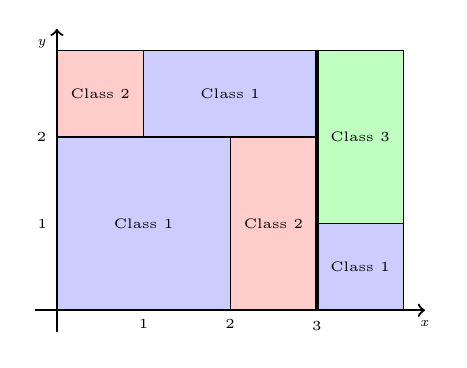
\begin{tikzpicture}[scale=1.1,font=\tiny]

            \draw[fill=red!20] (0,2) -- (1,2) -- (1,3) -- (0,3) -- cycle;

            \draw[fill=blue!20] (1,2) -- (3,2) -- (3,3) -- (1,3) -- cycle;

            \draw[fill=blue!20] (0,0) -- (2,0) -- (2,2) -- (0,2) -- cycle;
            \draw[fill=red!20] (2,0) -- (3,0) -- (3,2) -- (2,2) -- cycle;

            \draw[fill=blue!20] (3,0) -- (4,0) -- (4,1) -- (3,1) -- cycle;
            \draw[fill=green!25] (3,1) -- (4,1) -- (4,3) -- (3,3) -- cycle;

            \draw[->, thick] (-0.25,0) -- (4.25,0) node [below] {\textit{x}};
            \draw[->, thick] (0,-0.25) -- (0,3.25) node [below left] {\textit{y}};

            % decision lines

            \draw[line width=1.5pt,] (3,0) node [below] {3}  -- (3,3) ;
            \draw[line width=1pt] (0,2) node [left] {2} -- (3,2);

            \draw[] (2,0) node [below] {2}-- (2,2);

            \node [below] at (1,0) {1};

            \node [left] at (0,1) {1};

            % area labels
            \node [] at (0.5,2.5) {Class 2};
            \node [] at (2,2.5) {Class 1};

            \node [] at (1,1) {Class 1};
            \node [] at (2.5,1) {Class 2};


            \node [] at (3.5,2) {Class 3};
            \node [] at (3.5,0.5) {Class 1};

        \end{tikzpicture}
        \caption[Decision surface of the example decision tree]{The decision surface of the decision tree from \autoref{fig:decisionTreeExample} on $\mathcal{D}=[0,4]\times[0,3]$. }
        \label{fig:decisionBoundaryExample}
    \end{figure}
\end{multicols}


\subsection{Conversion of Decision Trees to Fuzzy Control Systems}

This section will demonstrate how to convert a classical decision tree into a fuzzy decision system using the fictional decision tree from \autoref{fig:decisionTreeExample} as an example.

\subsubsection{Fuzzy Decision Trees}

As the conversion makes use of so-called fuzzy decision trees, we will briefly introduce them here. Fuzzy decision trees are a generalization of classical decision trees and allow for fuzzy logic to be used in the decision-making process. Instead of following the classical \texttt{if then else} logic to descend into the decision tree, it uses fuzzy sets at each node of the tree to fuzzily calculate the contribution of each branch to the final decision based on the degree of truth of both possible paths. Contrary to classical decision trees, which follow a single path from the root to a leaf node, fuzzy decision trees explore all possible paths simultaneously and make a final decision by aggregating the results of the paths using fuzzy logic operations.

\subsubsection{Conversion}


A classical decision tree is converted into a fuzzy decision tree by replacing the crisp decision (e.g., $x \leq 3$) at each internal node of the decision tree with a fuzzy set. Those fuzzy sets should maintain the same semantics as the crisp decision but should provide a continuous value in the range $[0,1]$ specifying the degree of how much each branch should be considered. Classical decision trees can only make binary decisions (${0,1}$), which causes them to only consider a single path of the decision tree. Allowing them to consider multiple paths simultaneously can drastically increase the decision-making capabilities of the decision tree, especially in boundary cases where the decision can be ambiguous.


The shape of the membership functions of the fuzzy sets can be chosen arbitrarily, but since trees work with one-sided boundaries, typical choices include complementary \texttt{sigmoid}-shaped functions that are centered around the crisp decision boundary (See \autoref{fig:fuzzyMembershipFunctions}), as those function shapes maintain the semantics of the branching idea. Crockett et al.~\cite{CROCKETT20062809} suggested creating those sigmoid shapes with a \emph{width} proportional to the standard deviation of the attribute. In Particular, the authors suggested an interval $[t-n\cdot \sigma, t+n\cdot \sigma]$ for the membership function, where  $t$ is the value of the decision boundary, $\sigma$ is the standard deviation of the attribute and $n$ is a parameter that can be adjusted to control the \emph{width} of the membership function. This interval specifies the region of the membership function where most of the change in membership occurs. The value of $n$ is typically chosen from the interval $n\in [0,5]$ as the membership function can become too broad otherwise and could even weaken the decision-making process~\cite{CROCKETT20062809}. In this work, we will use $n=2$ as a default value. Using this method, it is possible to fully automate the conversion of a decision tree into a fuzzy decision tree, which we will utilize in this work.


\begin{figure}[h]
    \centering
    \begin{tikzpicture}[scale=2,font=\tiny]
        \node [rectangle,rounded corners,draw,inner sep=2pt] (A) at (0.5,0) {
            \crispTreeNode{x}{3}
        };

        \node [rectangle,rounded corners,draw,inner sep=2pt] (B) at (3.5,0) {
            \fuzzyTreeNode{x}{3}
        };

        \path[draw=black, line width=1mm, -{Triangle[length=4mm, bend]}]
        (1.5,0) to [bend left] (2.5,0);

        \path[draw=white, line width=0.5mm, -{Triangle[length=3.25mm, bend, angle'=60]}, shorten >= 0.5mm, shorten <= 0.25mm]
        (1.5,0) to [bend left] (2.5,0);

    \end{tikzpicture}
    \caption[Conversion of crisp tree node into fuzzy tree node]{Conversion of crisp set membership functions to fuzzy set membership functions. The classical membership functions $x \leq 3$ and $x>3$ of a decision tree node are replaced by two \texttt{sigmoid}-shaped membership functions \textcolor{red}{$\mu_{\text{xsmaller3}}$} and \textcolor{blue}{$\mu_{\text{xgreater3}}$} that specify to which degree one should traverse left or right. The \emph{width} of the membership functions is data dependent and is determined by $n\cdot \sigma = 2 \cdot \sigma$. }
    \label{fig:fuzzyMembershipFunctions}
\end{figure}

Once the internal nodes of the decision tree have been converted, the next step is to convert the leaf nodes of the decision tree to fuzzy leaf nodes. As the outputs of decision trees are specific class labels, we can define a single linguistic variable consisting of all possible class labels together with a corresponding fuzzy set. The shapes of the membership functions for the fuzzy sets can again be chosen mostly arbitrarily, but we will use \texttt{gaussian} functions with a different mean as they are a good choice for representing class labels in a continuous domain. This way of placing the fuzzy sets is not directly obvious, and the placement can significantly influence the defuzzification process depending on the chosen defuzzification function, as we will see later. However, we can minimize this issue by carefully choosing a suitable defuzzification method.
The resulting conversion of the decision tree in \autoref{fig:decisionTreeExample} into a fuzzy decision tree is shown in \autoref{fig:fuzzyDecisionTreeExample}.


\begin{figure}[h!]
    \centering
    \begin{tikzpicture}[scale=1.9,font=\tiny]

        \node [rectangle, rounded corners, draw, inner sep=2pt] (A) at (0,0) {
            \fuzzyTreeNode{x}{3}
        };

        \node [rectangle,rounded corners,draw,inner sep=2pt] (B) at (-2,-1.6) {
            \fuzzyTreeNode{y}{2}
        };

        \node [rectangle,rounded corners,draw,inner sep=2pt] (C) at (1.8,-1.6) {
            \fuzzyTreeNode{y}{1}
        };

        \node [rectangle,rounded corners,draw,inner sep=2pt] (D) at (-3,-3.2) {
            \fuzzyTreeNode{x}{2}
        };

        \node [rectangle,rounded corners,draw,inner sep=2pt] (E) at (-1,-3.2) {
            \fuzzyTreeNode{x}{1}
        };


        \node [rectangle,rounded corners,draw,inner sep=2pt,fill=blue!20] (F) at (-3.7,-4.7) {
            \fuzzyTreeLeaf{1}
        };

        \node [rectangle,rounded corners,draw,inner sep=2pt,fill=orange!20] (G) at (-2.6,-4.7) {
            \fuzzyTreeLeaf{2}
        };

        \node [rectangle,rounded corners,draw,inner sep=2pt,fill=orange!20] (H) at (-1.5,-4.7) {
            \fuzzyTreeLeaf{2}
        };

        \node [rectangle,rounded corners,draw,inner sep=2pt,fill=blue!20] (I) at (-0.4,-4.7) {
            \fuzzyTreeLeaf{1}
        };

        \node [rectangle,rounded corners,draw,inner sep=2pt,fill=blue!20] (J) at (1.25,-4.7) {
            \fuzzyTreeLeaf{1}
        };

        \node [rectangle,rounded corners,draw,inner sep=2pt,fill=green!20] (K) at (2.35,-4.7) {
            \fuzzyTreeLeaf{3}
        };



        \draw[->] (A) -- (B) node [pos=.4, left, above left] {yes};
        \draw[->] (A) -- (C) node [pos=.4, right, above right] {no};

        \draw[->] (B) -- (D) node [pos=.8, left, above left] {yes};
        \draw[->] (B) -- (E) node [pos=.8, right, above right] {no};

        \draw[->] (C) -- (J) node [pos=.2, left, above left] {yes};
        \draw[->] (C) -- (K) node [pos=.2, right, above right] {no};

        \draw[->] (D) -- (F) node [pos=.6, left, above left] {yes};
        \draw[->] (D) -- (G) node [pos=.6, right, above right] {no};

        \draw[->] (E) -- (H) node [pos=.6, left, above left] {yes};
        \draw[->] (E) -- (I) node [pos=.6, right, above right] {no};
    \end{tikzpicture}

    \caption[Fuzzy decision tree created from the regular decision tree]{The fuzzy decision tree corresponding to the decision tree in \autoref{fig:decisionTreeExample}. Internal nodes use two \texttt{sigmoid} membership functions (\textcolor{red}{$\mu_{\text{smaller}}$} and \textcolor{blue}{$\mu_{\text{greater}}$}) instead of a crisp decision. The leaf nodes use different \texttt{gaussian} membership functions centered around a unique mean.}

    \label{fig:fuzzyDecisionTreeExample}
\end{figure}

It is now possible to fully extract all linguistic variables from the fuzzy decision tree. Every fuzzy set defined over the same variable can be collected into a single linguistic variable. This results in linguistic variables consisting of a bunch of different \texttt{sigmoid} membership functions for input variables (internal nodes) and a single linguistic variable with different \texttt{gaussian} membership functions for the output variable (leaf nodes). The resulting linguistic variables are shown in \autoref{fig:fuzzyDecisionTreeLinguisticVariables}.


\begin{figure}[h]
    \centering

    \includegraphics[width=\linewidth]{figures/ProofOfConcepts/fuzzy_sets.png}

    \caption[Linguistic variables for the converted fuzzy decision tree]{Linguistic variables used in the fuzzy decision tree of \autoref{fig:fuzzyDecisionTreeExample}. The standard deviation of the attributes is assumed to be $\sigma \approx 0.5$ such that the \emph{width} of the sigmoid membership functions is $n\cdot \sigma \approx 1$. The standard deviation of the class values is chosen so that they do not overlap too much.}
    \label{fig:fuzzyDecisionTreeLinguisticVariables}
\end{figure}

\subsubsection{Rule Extraction}

The final step is to extract the fuzzy rules from the tree. This can be done by traversing the tree in a depth-first manner and collecting the correct membership functions for each path ending in a leaf node along the way. As all conditions of this path have to hold simultaneously, all fuzzy sets are connected using the \texttt{AND} operation. This newly created fuzzy set, which consists of the intersection of all fuzzy sets along the way, is the premise of selecting the fuzzy set of the leaf node. Consequently, both fuzzy sets are connected using the Mamdani \texttt{IMPLICATION} operator. This implication then forms a rule for the fuzzy system. Therefore, each unique path traversing the tree results in a unique rule. This process essentially mimics the decision surface seen in \autoref{fig:decisionBoundaryExample}, as we create precisely one rule for each region of the decision surface. The rules extracted from the fuzzy decision tree in \autoref{fig:fuzzyDecisionTreeExample} using this method are shown in \autoref{tab:fuzzyRulesExample}.


\newpage
\newcommand{\is}{\textit{ is }}


\begin{table}[H]
    \centering
    \begin{tabular}{c|l|c}
        \textbf{Rule} & \textbf{Antecedent}                                                             & \textbf{Consequent} \\
        \hline
        1             & $x \is \text{smaller3} \land y \is \text{smaller2} \land x \is \text{smaller2}$ & $class \is 1$       \\
        2             & $x \is \text{smaller3} \land y \is \text{smaller2} \land x \is \text{greater2}$ & $class \is 2$       \\
        3             & $x \is \text{smaller3} \land y \is \text{greater2} \land x \is \text{smaller1}$ & $class \is 2$       \\
        4             & $x \is \text{smaller3} \land y \is \text{greater2} \land x \is \text{greater1}$ & $class \is 1$       \\
        5             & $x \is \text{greater3} \land y \is \text{smaller1}$                             & $class \is 1$       \\
        6             & $x \is \text{greater3} \land y \is \text{greater1}$                             & $class \is 3$       \\
    \end{tabular}
    \caption[Extracted fuzzy rules from the fuzzy decision tree]{Extracted fuzzy rules from the fuzzy decision tree in \autoref{fig:fuzzyDecisionTreeExample} in the format: $\textbf{IF} \text{ Antecedent } \textbf{THEN} \text{ Consequent }$}
    \label{tab:fuzzyRulesExample}
\end{table}

\subsubsection{Fuzzy Control System}

With the linguistic variables and fuzzy rules extracted from the decision tree, we can finally use them to create a fuzzy system that can predict the class of a new data point based on its features. Since the fuzzy system can be seen as a black box mapping continuous input features to continuous output classes, we represent them as shown in \autoref{fig:fuzzyControlSystem} from now on. It is also possible to visualize the fuzzy system's decision surface by evaluating the system for each point in the input space, as shown in \autoref{fig:fuzzyDecisionSurface} for two different defuzzification methods. Such visualizations can help understand the decision-making process of the fuzzy system but, unfortunately, are not possible for higher-dimensional input spaces.


\begin{figure}[h]
    \centering
    \begin{tikzpicture}[scale=2,font=\small]

        \node [rectangle,rounded corners,draw,inner sep=2pt] (B) at (0,1.2) {
            Rules, Linguistic Variables \& Defuzzification Method
        };


        \node [rectangle, rounded corners, draw, inner sep=2pt,fill=white!80!black, fill ] (A) at (0,0) {
            \begin{tikzpicture}[scale=2,font=\tiny]
                \begin{axis}%
                    [
                        title={FCS},
                        width=3cm,
                        height=2cm,
                        axis lines=center,
                        xmin=0,
                        xmax=4,
                        xlabel={$\mathbb{R}$},
                        x label style={at={(axis description cs:1,0.2)},anchor=west},
                        ylabel=$\mu$,
                        y label style={at={(axis description cs:0,0.8)},anchor=east},
                        xtick={},
                        xticklabels= {},
                        ytick={},
                        yticklabels={},
                        ymax=1,
                        every axis plot/.append style={thick},
                        domain=0:4
                    ]
                    \addplot[blue, samples=17] {gaussian(x,1,0.2)};
                    \addplot[red,samples=15] {gaussian(x,2,0.2)};
                    \addplot[green,samples=17] {gaussian(x,3,0.2)};
                \end{axis}
            \end{tikzpicture}
        };



        \draw[->,thick] (B) -- (A);

        \draw[->,ultra thick] (-2.5,+0.2) -- (A) node [left, pos=0] {$x \in \mathbb{R}$};
        \draw[->,ultra thick] (-2.5,-0.2) -- (A) node [left, pos=0] {$y \in \mathbb{R}$};
        \draw[->,ultra thick] (A) -- (2.5,0) node [right, pos=1] {$class \in \mathbb{R}$};
    \end{tikzpicture}

    \caption[Fuzzy Control system created from the fuzzy decision tree seen as a black box]{The fuzzy control system created from the fuzzy decision tree in \autoref{fig:fuzzyDecisionTreeExample} can be seen as a black box that maps continuous input features to continuous output classes.}

    \label{fig:fuzzyControlSystem}
\end{figure}

\subsubsection{Choice of Defuzzification Method}

The exact shape of the decision surface depends on the specific defuzzification method used. The most common choice in literature is the \gls{cog} method, which calculates the $x$-position of the center of gravity of the membership function of the final fuzzy set.
However, using the \gls{cog} method can lead to undesired results when using nominal values for the output classes, which we will see later. The main problem is that the values have no concept of order. Without such an ordering, the interpolation between the different classes performed by methods such as \gls{cog} is not meaningful and leads to wrong predictions. Other methods, such as the \gls{mom} method, can be used instead. This method calculates the mean value of the maximum membership functions. In most cases, this method will return precisely the center of the membership function with the highest value and is a good choice for such types of knowledge bases. A direct comparison of the two methods on a critical datapoint is shown in \autoref{fig:fuzzySetForDataCOG} and \autoref{fig:fuzzySetForDataMOM}. Using the \gls{cog} method results in an opposite class than originally predicted from the fuzzy system, while the \gls{mom} method correctly predicts the class.

\begin{multicols}{2}

    \begin{figure}[H]
        \centering
        \includegraphics[width=0.9\columnwidth,trim={0 0 0 1cm},clip]{figures/ProofOfConcepts/fuzzy_set_for_data_cog.png}
        \caption[Resulting Fuzzy Set after applying the Rules on specific Data, COG Method]{Defuzzification on the fuzzy obtained by applying the rules from \autoref{tab:fuzzyRulesExample} on the data point $(x=2.95, y=2.5)$. There are clear peaks at the class values 1 and 3. However, the \gls{cog} method incorrectly suggests values close to class 2, thus turning the two good predictions into a bad one.}
        \label{fig:fuzzySetForDataCOG}
    \end{figure}

    \columnbreak

    \begin{figure}[H]
        \centering
        \includegraphics[width=0.9\columnwidth,trim={0 0 0 1cm},clip]{figures/ProofOfConcepts/fuzzy_set_for_data_mom.png}
        \caption[Resulting Fuzzy Set after applying the Rules on specific Data, MOM Method]{Defuzzification on the fuzzy obtained by applying the rules from \autoref{tab:fuzzyRulesExample} on the data point $(x=2.95, y=2.5)$. The \gls{mom} method correctly suggests the class value 1, as it is the class with the highest membership value.}

        \label{fig:fuzzySetForDataMOM}
    \end{figure}

\end{multicols}

As previously mentioned, we can recreate the process depicted in \autoref{fig:fuzzyControlSystem} for every possible input data point to visualize the fuzzy systems' decision surface. Both resulting decision surfaces are shown in \autoref{fig:fuzzySetForDataCOG} and \autoref{fig:fuzzySetForDataMOM}, respectively. The decision surface using the \gls{cog} tries to smoothly interpolate between the different classes, which causes interpolation errors if there are other classes in between. The decision surface using the \gls{mom} method is valid and closely resembles the decision surface of the crisp decision tree in \autoref{fig:decisionBoundaryExample}.

\begin{multicols}{2}
    \begin{figure}[H]
        \centering
        \begin{tikzpicture}
            \node[anchor=south west,inner sep=0] (image) at (0,0) { \includegraphics[width=0.9\columnwidth,trim={0 0 0 1.25cm},clip]{figures/ProofOfConcepts/fuzzy_system_cog.png}};
            \begin{scope}[x={(image.south east)},y={(image.north west)}]
                \draw[yellow, thin,rounded corners] (.55,.67) rectangle (.65,.95);
                \draw[yellow, thin,rounded corners] (.6,.32) rectangle (.74,.48);
                \node (A) at (.55,.56) [yellow, anchor=east] {\tiny{Interpolation Error}};

                \draw[yellow, arrow] (A) -- (.55,.67);
                \draw[yellow, arrow] (A) -- (.6,.48);
            \end{scope}
        \end{tikzpicture}

        \caption[Decision surface of the fuzzy rules using COG method]{Decision surface of the developed fuzzy-system using the \gls{cog} defuzzification method. The highlighted areas show interpolation errors caused by the defuzzification.}
        \label{fig:fuzzyDecisionSurfaceExampleCOG}
    \end{figure}

    \columnbreak

    \begin{figure}[H]
        \begin{tikzpicture}
            \node[anchor=south west,inner sep=0] (image) at (0,0) { \includegraphics[width=0.9\columnwidth,trim={0 0 0 1.25cm},clip]{figures/ProofOfConcepts/fuzzy_system_mom.png}};
        \end{tikzpicture}
        \caption[Decision surface of the fuzzy rules using MOM method]{Decision surface of the developed fuzzy-system using the \gls{mom} defuzzification method. There are no invalid regions in the decision surface.}
        \label{fig:fuzzyDecisionSurfaceExampleMOM}
    \end{figure}
\end{multicols}


\section{Fuzzy Control Systems for \texttt{md\_flexible}}

Following the fuzzy decision tree approach from the previous sections, we can create a fuzzy system to predict optimal configuration parameters for \texttt{\gls{mdflexible}} simulations. Contrary to the previous example, we must first collect a dataset of simulation runs with different configuration parameters and their corresponding performance metrics, which can then be used to train the crisp decision tree. After converting the crisp decision tree to a \gls{fcs}, a human expert can evaluate and adjust the rules and membership functions if necessary.

The resulting fuzzy system can then be used to predict the optimal configuration parameters for new simulation runs based on the current state of the simulation.

\subsection{Data Collection}

Using the \texttt{LiveInfoLogger} and \texttt{TuningDataLogger} classes of the \gls{autopas} framework, it is possible to collect all the necessary data needed to train the decision tree. Both loggers create a \texttt{.csv} file containing each tuning step's simulation parameters and current runtime results. The \texttt{LiveInfoLogger} logs summary statistics about the simulation state, such as the average number of particles per cell or the current homogeneity-estimation of the simulation. In contrast, the \texttt{TuningDataLogger} logs the current configuration and the time it took to execute the last tuning step. The complete list of currently available parameters and their descriptions can be found in \autoref{des:liveinfodatafields} and \autoref{des:tuningdatafields}, respectively.

We will only make use of a subset, however, as we are only interested in \emph{relative} values, that does not change when the simulation is scaled up or down and are therefore only include:  \texttt{avgParticlesPerCell}, \texttt{maxParticlesPerCell}, \texttt{homogeneity}, texttt{maxDensity}, \texttt{particlesPerCellStdDev} and \texttt{threadCount}.

All the values were collected with the \texttt{PAUSE\_SIMULATION\_DURING\_TUNING} cmake option enabled to ensure that the simulation state does not change during the tuning process. This ensures a fair comparison of the different configurations, as all of them are evaluated under the same conditions.

The data was collected on the CoolMUC-2 \todo{add specs} and primarily stems from the example scenarios provided by \gls{mdflexible} such as \texttt{explodingLiquid.yaml}, \texttt{fallingDrop.yaml}, \texttt{SpinodalDecomposition.yaml} and some simulations of uniform cubes with different particle counts and densities. The exact scenarios files used for the simulations can be found in \autoref{des:scenarios}.
All simulations were run on the serial partition of the cluster and were repeated twice to account for fluctuations in performance. Furthermore, every simulation was run with 1, 4, 12, 24, and 28 threads to gather data on how parallelization affects the ideal configuration.


\subsection{Speedup Analysis}

In order to make predictions about the performance of different configurations, we first need to define the metric used to compare them. As we froze the simulation during the tuning process, we can safely use the runtime of configuration during a tuning phase to find an ordering. To make these timings comparable between tuning phases, we introduce the term \emph{relative speedup}. The relative speedup describes the performance of a configuration relative to the best configuration in the tuning phase. The formula for the relative speedup is given by:

\begin{equation}
    {\text{speedup}^{(i)}_{\text{config}}}= \frac{t_{\text{best}}^{(i)}}{t_{\text{config}}^{(i)}}
\end{equation}

Where $t_{\text{best}}^{(i)}$ is the runtime of the best configuration during the $i$-th tuning phase and $t_{\text{config}}^{(i)}$ is the runtime of the configuration we are interested in.

This means that all relative speedup values are going to be in the range $[0,1]$, with 1 being the best possible value only achieved by configurations performing optimally and 0 being the worst possible value only achieved by configurations performing \emph{infinitely} worse than the best configuration.

We can then make plots of the distribution of the relative speedup values for each configuration option to see how they affect the performance of the simulation. The density plots in \autoref{fig:inputAnalysisDensityNewton3}, \autoref{fig:inputAnalysisDensityTraversal}, \autoref{fig:inputAnalysisDensityDatalayout} and \autoref{fig:inputAnalysisDensityConfigurations} show the distribution of the relative speedup values for the Newton3, Traversal, Container-Datalayout and some complete configurations respectively. We can see that the Newton3 option generally leads to a higher relative speedup, while the Traversal option does not show a clear trend. The Datalayout option shows that the VerletListCells\_AoS option is generally the best, while the configuration VerletListCells\_AoS\_vlc\_spliced\_balanced\_enabled is the best configuration in most cases on the Dataset we collected.

The ordering of the different parameters in the dataset matches our intuition about the different implementations, and we can confidently proceed with creating the fuzzy system.



\subsection{Creating the Fuzzy Rules}

Using the decision tree approach described in the previous sections, we can create a fully automated system to transform the collected data into rule files. The process is as follows:

\begin{enumerate}
    \item Preprocess the data according to the approach used (see next section).
    \item Train the decision trees and prune the tree to avoid overfitting.
    \item Select the best-performing decision trees and convert them into fuzzy decision trees.
    \item Extract the fuzzy rules from the fuzzy decision trees.
    \item Generate the linguistic variables and terms for the fuzzy system.
    \item Create the OutputMapping Export and export everything to a rulefile.
\end{enumerate}

As described previously, we will create two different kinds of knowledge bases, one for the Suitability Approach and one for the Individual Tuning Approach. In the following sections, we will describe both approaches in detail.

\subsection{Individual Tuning Approach}

This approach tries to create different fuzzy systems for each of the tunable parameters of the simulation. We decided to combine the \texttt{container} and \texttt{dataLayout} parameters into a single parameter as they are closely related, and the performance of one is heavily dependent on the other. Consequently, we want to create systems for \texttt{ContainerDataLayout}, \texttt{Traversal}, and \texttt{Newton3}.

As we only want to create a fuzzy system predicting suitable configurations, we first remove all configurations performing worse than a certain threshold as depicted in \autoref{fig:speedup}. We chose to only include configurations with a relative speedup of at least 70\% % as this still leaves us with a large enough dataset to train the decision trees.

\begin{figure}[H]
    \centering
    \includegraphics[width=\columnwidth,trim={1cm 0 2cm 1.5cm},clip]{figures/DataAnalytics/speedup.png}
    \caption[Speedup density plot of all configurations]{The density plot shows the distribution of all the collected configurations concerning the relative speedup compared to the best configuration during each tuning phase. This distribution shows that the average tested configuration performs just 50\% as well as the best. With some configurations being ten times slower than the best configuration.
        Efficiently finding good configurations is key, as testing all possible configurations causes a huge performance loss.}
    \label{fig:speedup}
\end{figure}

Afterward, we group all configurations evaluated in the same tuning phase and aggregate all the present values of tunable parameters into a single term. This term represents all \emph{good} values for the parameters to be chosen under the conditions of the tuning phase. The resulting training data is shown in \autoref{tab:trainingDataIndividual} and can be used to train the decision trees. After applying the transformation process described in the previous sections, we end up with rules shown in \autoref{tab:fuzzyRulesIndividual}. This concludes the creation of the fuzzy rules for the Individual Tuning Approach.




\begin{table}[H]
    \footnotesize
    \centering
    \begin{tabular}{|c|c|c|c|c|}
        \hline

        \textbf{LiveInfo Data} & \textbf{Container\_DataLayout} & \textbf{Traversal} & \textbf{Newton3} \\
        \hline
        \makecell{(0.905797,	0.055112,                                                                   \\	0.297891,	15,	0.015171,	4) }                                                                                                              & \makecell{"LinkedCells\_SoA,                                                \\ VerletClusterLists\_SoA, \\ VerletListsCells\_AoS"} & \makecell{"lc\_sliced,\\ lc\_sliced\_balanced,\\ lc\_sliced\_c02,\\ lc\_c04"} & "enabled"          \\
        \hline
        \makecell{(0.944637,	0.084061,                                                                   \\	0.673320,                                                                                                                                                                                                   	25,	0.039916, 24) }                                                                                                               & \makecell{"LinkedCells\_SoA,                                                \\ VerletClusterLists\_SoA, \\ VerletListsCells\_AoS"} & \makecell{"lc\_c04,\\ lc\_c08,\\ lc\_sliced,\\ lc\_sliced\_balanced"} &  \makecell{"disabled,\\enabled"}         \\
        \hline
        \makecell{(0.905797,	0.041394,                                                                   \\	0.336900,                                                                                                                                                                                                   	20,	0.013546, 24) }                                                                                                               & \makecell{"VerletClusterLists\_SoA,                                         \\ VerletListsCells\_AoS"} & \makecell{"vcl\_c06,\\ vlc\_c01,\\ vlc\_c18,\\ vlc\_sliced\_c02"} &  \makecell{"disabled,\\enabled"}         \\
        \hline

        \vdots                 & \vdots                         & \vdots             & \vdots           \\
        \hline
    \end{tabular}
    \caption[Prepared training data for the Individual Tuning Approach]{Selection of the prepared training data for the Individual Tuning Approach. The table shows the live info data and the corresponding prediction of top-performing values for each tunable parameter. Each row represents a different tuning phase.}
    \label{tab:trainingDataIndividual}
\end{table}




\definecolor{LightCyan}{rgb}{0.88,1,1}
\newcolumntype{g}{>{\columncolor{LightCyan}}c}

\begin{table}[H]
    \footnotesize
    \centering
    \addtolength{\leftskip} {-3cm} % increase (absolute) value if needed
    \addtolength{\rightskip}{-3cm}

    \begin{tabular}{|c|c|c|c|g|}
        \multicolumn{4}{c}{\large{\textbf{Antecedent}}} & \multicolumn{1}{c}{\large{\textbf{Consequent}    }}                                                                                                                                    \\
        \hline
        \textbf{avgParticlesPC}                         & \textbf{homogeneity}                                & \textbf{particlesPCStdDev}                        & \textbf{threadCount}      & \textbf{ContainerDataLayout}                     \\

        \hline
        \texttt{lower than 3.454}                       & \texttt{lower than 0.05}                            &                                                   & \texttt{lower than 18.0}  & \tabularCenterstack{c}{"VerletClusterLists\_SoA, \\
        VerletListsCells\_AoS"}                                                                                                                                                                                                                  \\
        \hline
        \texttt{lower than 3.454}                       & \texttt{higher than 0.05}                           & \texttt{lower than 0.024}                         & \texttt{higher than 18.0} & \tabularCenterstack{c}{"LinkedCells\_SoA,        \\ VerletClusterLists\_SoA,\\ VerletListsCells\_AoS"}  \\
        \hline
        \vdots                                          & \vdots                                              & \vdots                                            & \vdots                    & \vdots                                           \\
        \hline

        \multicolumn{5}{c}{ }                                                                                                                                                                                                                    \\


        \multicolumn{4}{c}{\large{\textbf{Antecedent}}} & \multicolumn{1}{c}{\large{\textbf{Consequent}    }}                                                                                                                                    \\

        \hline
        \textbf{avgParticlesPC}                         & \textbf{homogeneity}                                & \textbf{particlesPCStdDev}                        & \textbf{threadCount}      & \textbf{Traversal}                               \\

        \hline

        \texttt{lower than 1.553}                       & \texttt{higher than 0.047}                          & \texttt{lower than 0.023	}                         & \texttt{higher than 2.5}  & \tabularCenterstack{c}{"lc\_sliced,              \\ vlc\_c18,\\ lc\_sliced\_c02"}
        \\
        \hline

                                                        & \texttt{lower than 0.037}                           & \texttt{lower than 0.023	}                         & \texttt{lower than 26.0}  & \tabularCenterstack{c}{"vcl\_c06,                \\ vlc\_c18,\\ vlc\_sliced\_c02"}                                                          \\


        \hline
        \vdots                                          & \vdots                                              & \vdots                                            & \vdots                    & \vdots                                           \\
        \hline


        \multicolumn{5}{c}{ }                                                                                                                                                                                                                    \\


        \multicolumn{4}{c}{\large{\textbf{Antecedent}}} & \multicolumn{1}{c}{\large{\textbf{Consequent}    }}                                                                                                                                    \\

        \hline
        \textbf{avgParticlesPC}                         & \textbf{homogeneity}                                & \textbf{particlesPCStdDev}                        & \textbf{threadCount}      & \textbf{Newton 3}                                \\

        \hline

                                                        &                                                     & \texttt{higher than 0.03}                         & \texttt{higher than 18.0} & \tabularCenterstack{c}{"disabled,                \\enabled"}
        \\
        \hline

                                                        &                                                     & \tabularCenterstack{c}{\texttt{higher than 0.023}                                                                                \\ $\land$ \texttt{lower than 0.037	}} &  \tabularCenterstack{c}{\texttt{lower than 18.0}\\ $\land$ \texttt{higher than 8.0	}} & \tabularCenterstack{c}{"enabled"}                \\


        \hline
        \vdots                                          & \vdots                                              & \vdots                                            & \vdots                    & \vdots                                           \\
        \hline
    \end{tabular}

    \caption[Extracted fuzzy rules for the Individual Tuning Approach]{Extracted fuzzy rules for the Individual Tuning Approach. The table shows a selection of the rules extracted from the decision trees trained on the training data in \autoref{tab:trainingDataIndividual}. The columns of the antecedent represent the different fuzzy sets taking part in the rule.}
    \label{tab:fuzzyRulesIndividual}
\end{table}


We can also visualize the training data in a scatterplot as shown in \autoref{fig:scatterContainerDataLayout}.

% scatter_container_datalayout

\begin{figure}[H]
    \centering
    \includegraphics[height=8cm,trim={0cm 0.7cm 1cm 1.5cm},clip]{figures/DataAnalytics/scatter_container_datalayout.png}
    \caption[Scatterplot of the ContainerDataLayout parameter]{The scatterplot shows the influence of the variables \texttt{homogeneity}, \texttt{particlesPerCellStdDev} and \texttt{threadCount} on the optimal \texttt{ContainerDataLayout} parameter. We can see regions that will be learned by the decision tree.}
    \label{fig:scatterContainerDataLayout}

\end{figure}



As described previously, we use \texttt{gaussian} membership functions for each linguistic term of the consequent linguistic variables. The placement of the  values is irrelevant, and we place them in a way that does not overlap. \autoref{fig:homogenityLinguisticVariable} and \autoref{fig:newton3LinguisticVariable_individual} show the resulting linguistic variables for an antecedent linguistic variable (homogeneity) and a consequent linguistic variable (Newton3), respectively. The visualization of the other variables follows a similar pattern but is more complex due to the higher number of terms, which are therefore not shown here.



\begin{multicols}{2}
    \begin{figure}[H]
        \centering
        \includegraphics[width=\columnwidth,trim={1cm 0 1cm 1.35cm},clip]{figures/DataAnalytics/homogenity_linguistic_variable.png}

        \caption[Linguistic variable for the homogeneity attribute]{
            This figure shows the linguistic variable for the homogeneity attribute. We see the different fuzzy sets created from the decision trees. The background shows the histogram of all homogeneity values present in the dataset.
        }
        \label{fig:homogenityLinguisticVariable}
    \end{figure}

    \columnbreak

    \begin{figure}[H]
        \includegraphics[width=\columnwidth,trim={1cm 0 1cm 1.35cm},clip]{figures/DataAnalytics/newton3_linguistic_variable.png}
        \caption[Linguistic variable for the Newton3 attribute]{
            This figure shows the linguistic variable for the Newton3 attribute. We see the two \texttt{gaussian} membership functions representing the two possible values for the Newton3 attribute.
        }
        \label{fig:newton3LinguisticVariable_individual}
    \end{figure}
\end{multicols}

At the end of the process, we have different fuzzy systems for each of the tunable parameters of the simulation of the form shown in \autoref{fig:fuzzyControlSystemIndividual}. The fuzzy system can be seen as a black box that maps the LiveInfo data into a sort of \emph{index} representing the predicted values of the parameter. Using the \gls{mom} method, the output will always correspond to the fuzzy set with the highest membership value and be free of interpolation errors.


\subsection{Suitability Approach}

The suitability approach differs from the individual tuning approach in that it tries to predict a configuration's numerical \emph{suitability} value under the current conditions. Therefore, each possible configuration is assigned a unique fuzzy system tailored to just evaluating this configuration—the suitability value of a configuration defined as the relative speedup already described in the previous section.

The process is similar to the one described in the previous section. However, we do not group the configurations together and directly use the calculated relative speedup as the suitability value.

To train the decision trees, we again use a classification-based approach with \texttt{terrible}, \texttt{bad}, \texttt{average}, \texttt{good}, and \texttt{excellent} as the possible linguistic terms (see \autoref{fig:suitabilityClasses}). The calculated suitability values of each configuration during a specific tuning phase are mapped to the corresponding class.

The final training data is shown in \autoref{tab:trainingDataSuitability}, and it is again possible to train the decision trees and extract the fuzzy rules from them. It is important to note that each configuration has its own fuzzy system and rules tailored to it. This makes the suitability approach more flexible but also causes more computational overhead during the inference process.

The resulting rules are shown in \autoref{tab:fuzzyRulesSuitability}, and the linguistic variables for the suitability attribute are shown in \autoref{fig:suitabilityClasses}. The output mapping for the suitability approach is shown in \autoref{lst:outputMappingSuitability}.

\begin{figure}[H]
    \centering
    \includegraphics[width=\columnwidth,trim={1cm 0 2cm 1.5cm},clip]{figures/DataAnalytics/membership_suitability_config.png}
    \caption[Linguistic variable for the Suitability attribute]{
        Linguistic terms for the suitability variables. The fuzzy sets consist of  \texttt{sigmoid} membership functions at the borders and \texttt{gaussian} membership functions in the middle. The values are placed coherently. This time, we will use the \gls{cog} defuzzification method and will make use of the interpolation between the values.
    }
    \label{fig:suitabilityClasses}
\end{figure}


\begin{table}[H]
    \footnotesize
    \centering
    \begin{tabular}{|c|c|c|c|c|}
        \hline

        \textbf{LiveInfo Data} \footnote{
            The format of the LiveInfo tuple is: (avgParticlesPC, homogeneity, maxDensity,particlesPerCellStdDev, threadCount)
        }      & \textbf{Configuration} \footnote{
            The format of the Configuration is: Container, DataLayout, Traversal, Newton3
        }      & \textbf{Speedup}                  & \textbf{Suitability}          \\
        \hline
        \makecell{(0.905797,	0.035496,                                              \\	0.531948,	0.012989,	1) }                                                                                                              & \makecell{LinkedCells, AoS, lc\_sliced, enabled} &0.450641 & "bad"          \\
        \hline
        \makecell{(0.944637,	0.083797,                                              \\	0.691920	,	0.012989,	28) }                                                                                                              & \makecell{VerletClusterLists, AoS,vcl\_c06, disabled} &0.319094	 & "rubbish"          \\
        \hline
        \makecell{(0.944637,	0.079441,                                              \\	0.040082	,	0.012989,	12) }                                                                                                              & \makecell{LinkedCells, SoA,lc\_sliced, c02,enabled} &0.989101 & "excellent"          \\
        \hline

        \vdots & \vdots                            & \vdots               & \vdots \\
        \hline
    \end{tabular}
    \caption[Prepared training data for the Individual Tuning Approach]{Selection of the prepared training data for the Individual Tuning Approach. The table shows the live info data and the corresponding prediction of top-performing values for each tunable parameter. Each row represents a different tuning phase.}
    \label{tab:trainingDataSuitability}
\end{table}




\definecolor{LightCyan}{rgb}{0.88,1,1}
\newcolumntype{g}{>{\columncolor{LightCyan}}c}

\begin{table}[H]
    \footnotesize
    \centering
    \addtolength{\leftskip} {-3cm} % increase (absolute) value if needed
    \addtolength{\rightskip}{-3cm}

    \begin{tabular}{|c|c|c|c|g|}
        \multicolumn{4}{c}{\large{\textbf{Antecedent}}} & \multicolumn{1}{c}{\large{\textbf{Consequent}    }}                                                                                                                                  \\
        \hline
        \textbf{avgParticlesPC}                         & \textbf{homogeneity}                                & \textbf{particlesPCStdDev} & \textbf{threadCount}                              & \textbf{ LinkedCells\_AoS\_lc\_c01\_disabled} \\

        \hline
                                                        & \texttt{lower than 0.084}                           & \texttt{higher than 0.029} & \texttt{higher than 26.0 }                        & "medium"                                      \\
        \hline
                                                        & \texttt{higher than 0.084}                          & \texttt{higher than 0.029} & \texttt{higher than 26.0 }                        & "bad"                                         \\
        \hline
                                                        &                                                     & \texttt{higher than 0.02}  & \texttt{lower than 2.5	 }                          & "rubbish"                                     \\

        \hline
        \vdots                                          & \vdots                                              & \vdots                     & \vdots                                            & \vdots                                        \\
        \hline

        \multicolumn{5}{c}{ }                                                                                                                                                                                                                  \\


        \multicolumn{4}{c}{\large{\textbf{Antecedent}}} & \multicolumn{1}{c}{\large{\textbf{Consequent}    }}                                                                                                                                  \\

        \hline
        \textbf{maxParticlesPerCell}                    & \textbf{homogeneity}                                & \textbf{particlesPCStdDev} & \textbf{threadCount}                              & \textbf{ LinkedCells\_AoS\_lc\_c04\_disabled} \\

        \hline
        \texttt{higher than 18.5	}                       & \texttt{lower than 0.082}                           &                            & \tabularCenterstack{c} {\texttt{higher than 18.0}                                                 \\ $\land$ \texttt{ lower than 26.0}} & "medium" \\

        \hline
        \texttt{higher than 18.5	}                       & \texttt{higher than 0.082}                          &                            & \tabularCenterstack{c} {\texttt{higher than 18.0}                                                 \\ $\land$ \texttt{ lower than 26.0}} & "bad" \\
        \hline


        \vdots                                          & \vdots                                              & \vdots                     & \vdots                                            & \vdots                                        \\

        \hline
    \end{tabular}

    \caption[Extracted fuzzy rules for the Suitability Approach]{Extracted fuzzy rules for the Suitability Approach. The table shows a selection of the rules extracted from the decision trees trained on the training data in \autoref{tab:trainingDataSuitability}. The columns of the antecedent represent the different fuzzy sets taking part in the rule.}
    \label{tab:fuzzyRulesSuitability}
\end{table}



